\section{Chunkwise WY form and the TPU kernels}
\label{sec:kernels}

Equation~\eqref{eq:kda} is a sequential recurrence; trained naively it
serializes 2048 steps. The training path instead processes the sequence
in chunks of $C = 64$, expressing everything inside a chunk with dense
matrix algebra (which TPUs execute at full matrix-unit utilization) and
carrying the fast-weight state only across chunk boundaries.

\subsection{Chunkwise decomposition}

Write $G_i = \sum_{s \le i} g_s \in \R^{d_k}$ for the inclusive
cumulative log-decay within a chunk. Unrolling \eqref{eq:kda} from the
chunk-entry state $S$ gives, for the output at intra-chunk position $i$,
a \emph{cross-chunk} term read through the accumulated decay and an
\emph{intra-chunk} term over earlier positions of the same chunk:
\begin{equation}
o_i \;=\; \big(q_i \odot e^{G_i}\big)^{\top} S
\;+\; \sum_{j \le i} \Xi_{ij}\, \hat{v}_j,
\qquad
\Xi_{ij} = \big\langle q_i \odot e^{G_i - G_j},\, k_j \big\rangle ,
\label{eq:chunk-out}
\end{equation}
where the $\hat{v}_j$ are \emph{delta-corrected} values: the values
actually written to the state after subtracting the state's own
prediction. The corrections inside one chunk satisfy a unit-lower-
triangular linear system. Defining the decay-weighted Gram matrix
$M_{ij} = \langle \beta_i k_i \odot e^{G_i - G_j},\, k_j\rangle$ for
$j < i$ and $T = \mathrm{StrictLower}(M)$,
\begin{equation}
(I + T)\, U = B_v, \qquad (I + T)\, W = B_k,
\label{eq:wy-solve}
\end{equation}
with $B_v = [\beta_i v_i]_i$ and $B_k = [\beta_i k_i \odot e^{G_i}]_i$.
This is the WY representation of the product of rank-one delta updates:
$U$ and $W$ compress the chunk's 64 sequential writes into two dense
matrices. The corrected values and the state advance are then
\begin{equation}
\hat{V} = U - W S,
\qquad
S \leftarrow \diag\!\big(e^{G_C}\big)\, S
+ \big(k \odot e^{G_C - G}\big)^{\top} \hat{V},
\label{eq:chunk-scan}
\end{equation}
one dense contraction per chunk, with $S$ the only sequential carrier.

\subsection{Decay-anchored pairwise dots and the overflow bound}
\label{sec:pairwise}

Every matrix above contains entries of the form
\begin{equation}
M_{ij} \;=\; \sum_{d} L_{i,d}\, R_{j,d}\, e^{G_{i,d} - G_{j,d}},
\label{eq:pairwise}
\end{equation}
which cannot be computed as a plain matmul because the decay factor
depends on \emph{both} indices and on the channel. Materializing the
$[C, C, d_k]$ tensor is prohibitive; factorizing
$e^{G_i - G_j} = e^{G_i} e^{-G_j}$ overflows, since $-G_j$ can reach
$|\ell| \cdot C = 320$ and $e^{320}$ is far beyond fp32.

The kernel factorizes against a moving \emph{anchor} instead. Rows are
processed in blocks of $R$ rows; each block is anchored at its last
row's cumulative decay $a = G_{\text{block end}}$:
\begin{equation}
M_{ij} = \sum_d
\underbrace{\big(L_{i,d}\, e^{G_{i,d} - a_d}\big)}_{\text{left factor}}
\cdot
\underbrace{\big(R_{j,d}\, e^{a_d - G_{j,d}}\big)}_{\text{right factor}},
\end{equation}
a true matmul per block. The anchor cancels exactly in the product. The
right factor's exponent $a_d - G_{j,d}$ is nonpositive for every valid
column ($j$ at or before the anchor), so the right factor never exceeds
1; the left factor's exponent spans at most the $R$ rows of one block.
Since $g \in (\ell, 0)$ with $\ell = -5$
(Eq.~\ref{eq:safe-gate}), the one-sided exponent obeys
\begin{equation}
\max_{i,d} \left| G_{i,d} - a_d \right| \;\le\; |\ell| \cdot R
\;=\; 5 \cdot 16 = 80,
\qquad
e^{80} \approx 5.5 \times 10^{34} \;<\; 3.4 \times 10^{38} = \text{fp32 max}.
\label{eq:overflow-bound}
\end{equation}
This inequality is checked at kernel import time. It is why the gate
bound $\ell = -5$ is a \emph{kernel compute parameter}: relaxing the
gate below $-5$, or widening the row block past 16 with last-row
anchoring, breaks \eqref{eq:overflow-bound} and the kernel refuses to
build. (Anchoring at the block midpoint would halve the one-sided
exponent and double the admissible block; the production kernels use
$R = 8$ on v5e/v6e and $R = 16$ on v4, both comfortably inside the
bound.) Invalid future columns are set to $-\infty$ \emph{before}
exponentiation --- masking after the fact would leave overflowed values
in the backward graph.

\subsection{The WY solve: a divide-and-conquer nilpotent inverse}
\label{sec:inverse}

System \eqref{eq:wy-solve} is a unit-lower-triangular solve of size
$C = 64$ against a 256-wide right-hand side. Forward substitution is
stable but latency-bound on a TPU: ~60 chained small matmuls per solve.
The production kernel forms the explicit inverse instead, by
divide and conquer. Split
\begin{equation}
I + T =
\begin{pmatrix} A_{11} & 0 \\ A_{21} & A_{22} \end{pmatrix},
\qquad
(I+T)^{-1} =
\begin{pmatrix} A_{11}^{-1} & 0 \\
-A_{22}^{-1} A_{21} A_{11}^{-1} & A_{22}^{-1} \end{pmatrix}.
\end{equation}
Writing $M$ for the block-diagonal matrix of the two inverted halves and
$C_\times$ for the pre-multiplied coupling block, the merge step is the
closed form
\begin{equation}
\boxed{\;(I+T)^{-1} \;=\; M - M\, C_\times\, M\;}
\label{eq:dc-inverse}
\end{equation}
\begin{proposition}
Equation \eqref{eq:dc-inverse} is exact, not a truncation.
\end{proposition}
\begin{proof}
$M C_\times M$ has only a lower-left block, so $(M C_\times M) C_\times
(M \cdot) = 0$: the coupling is nilpotent of index two, and the Neumann
series $M - M C_\times M + M C_\times M C_\times M - \cdots$ terminates
after its second term.
\end{proof}
Base blocks of size 2 invert as $I - T_{2}$ with no arithmetic at all;
five merge levels build the full $64 \times 64$ inverse in ten uniform
matmuls, and applying it to the right-hand side is a single dense
matrix-unit contraction. Two alternatives were implemented and rejected
by measurement: blocked forward \emph{substitution} (stable, $-30\%$
end-to-end throughput) and a \emph{repeated-squaring} Neumann form whose
intermediate powers $T^2, T^4, \ldots, T^{32}$ grow to $\sim 10^{12}$ on
real-text keys and destroy the backward pass by cancellation
(\S\ref{sec:numerics}).

\subsection{The fused kernels}

The production kernel fuses the entire mixer --- causal conv, SiLU,
normalization, cumulative decay, pairwise dots, the solve, and the
chunk scan --- into one Pallas program per (batch, chunk-stream): grid
$(B, T/C)$ with the chunk axis sequential, all heads processed together,
the $H \times 128 \times 128$ fp32 state and the $w{-}1$ rows of
convolution history resident in VMEM across chunk iterations. XLA never
materializes a convolved, activated, split, or head-transposed copy of
the QKV projections; the kernel consumes the raw $[B, T, 3, H, D]$
projection output and emits bf16 outputs plus an fp32 state history
(one snapshot per chunk) for the backward.

The backward is a second fused kernel running the grid in reverse: it
recomputes each chunk's forward quantities from the raw projections,
carries $\bar{S}$ in VMEM, threads the $w{-}1$ \emph{future} rows of
convolution cotangents backward through a scratch ring, and applies
hand-derived adjoints for every stage --- including a blockwise VJP of
\eqref{eq:pairwise} that never materializes the $[C, C, d_k]$ tensor,
the solve adjoint
$\bar{T} = -\mathrm{tril}\big(A^{-\top}\bar{A}A^{-\top}, -1\big)$,
and a reverse cumulative sum taking $\bar{G}$ back to $\bar{g}$.

\paragraph{TPU v4 variant.} The folded kernel's in-kernel
$[\mathrm{time},\mathrm{head}]$ transposes lower to sublane gathers that
the v4 compiler backend rejects, so v4 runs a pre-fold variant: the QKV
mixer stays in XLA and the backward is \emph{split into two kernels} at
the solve/pairwise boundary --- a reverse sequential stage exporting
per-chunk partials to HBM, then a chunk-parallel epilogue. On the
campaign hardware the three KDA kernel launches together account for
$\sim$15\% of the training step; the dense GEMM body dominates.

\begin{table}[h]
\centering
\small
\caption{Kernel generations on the 273M-class hybrid, TPU v6e-8, batch 8
$\times$ 2048. ``Core'' is the isolated KDA forward+backward.}
\label{tab:kernels}
\begin{tabular}{lrr}
\toprule
 & core fwd+bwd & full-model throughput \\
\midrule
analytical XLA backward & 31.9 ms & 514k tok/s (core) \\
fused Pallas, substitution solve & --- & 473k tok/s \\
fused Pallas, divide-and-conquer inverse & 5.0 ms & \textbf{616k tok/s} \\
\midrule
blanket one-pass bf16 (rejected) & 4.9$\times$ faster core & NaN by step 2 \\
\bottomrule
\end{tabular}
\end{table}

\begin{figure}[t]
\centering
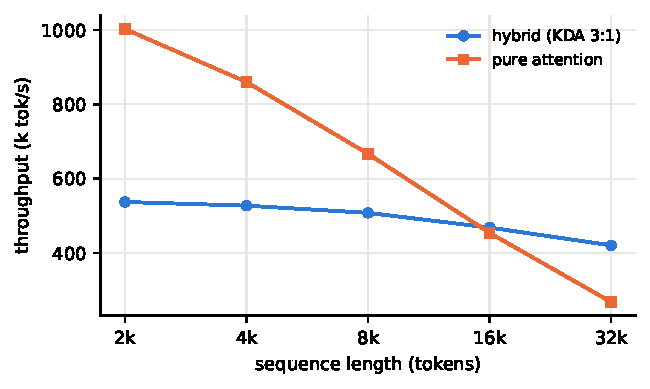
\includegraphics[width=0.62\textwidth]{figures/seq_sweep.pdf}
\caption{Throughput vs.\ sequence length, hybrid (3:1 KDA) against a
pure-attention control of the same size (TPU v6e-8). The recurrent
layers' linear scaling overtakes quadratic attention near 16k tokens;
at 32k the hybrid is $1.6\times$ faster. At the campaign's 2048 the
hybrid pays $\sim$2$\times$ for its richer mixer --- the price of buying
long-context headroom at training time.}
\label{fig:seqsweep}
\end{figure}
